\section{MCCFR: learn from dealt hands instead of enumerating the universe}\label{sec:mccfr}

\mkey{monte carlo cfr}Vanilla CFR's iteration cost is the whole tree, and Drawmaha's tree is dominated by chance: $\approx 4.0\times10^{12}$ ways to deal the two starting hands, before boards and replacement cards. \keyterm{Monte Carlo CFR}\mdef{MCCFR}{sample part of the tree each iteration; update visited infosets with estimates that are correct on average} (Lanctot et al.\ 2009)~\cite{lanctot2009} replaces ``enumerate every deal'' with ``play sessions'': each iteration samples a slice of the tree and updates only the infosets it visits, using estimates constructed to equal the full-CFR update \emph{in expectation}. Convergence survives (with high probability); iterations get cheaper by orders of magnitude; you take many more of them and win on wall-clock.

The design space is \emph{what to sample}, and Figure~\ref{fig:sampling} draws the two poles:

\begin{figure}[t]
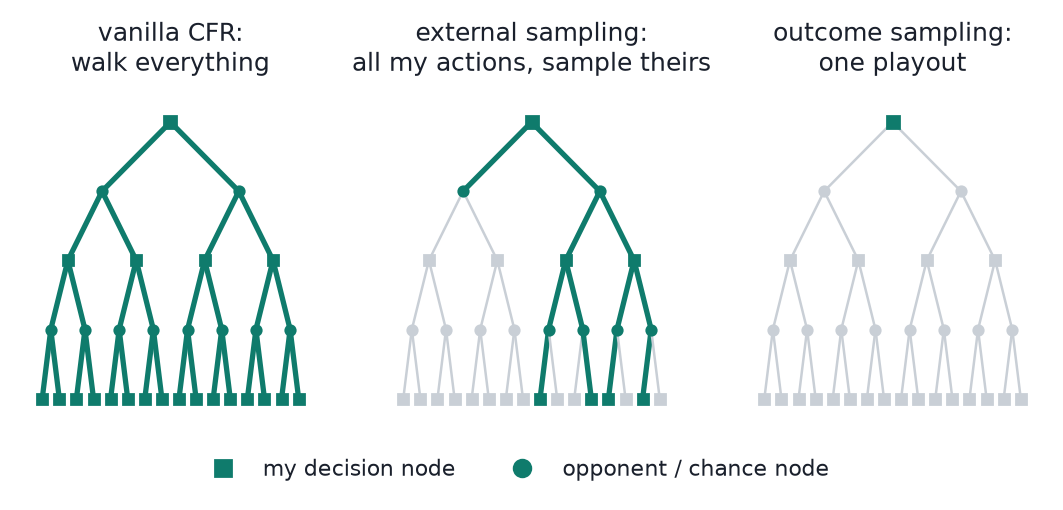
\includegraphics[width=\linewidth]{figures/sampling.png}
\caption{What one iteration touches under each traversal scheme (teal = visited).}
\label{fig:sampling}
\end{figure}

\begin{itemize}
\item \keyterm{External sampling}\mdef{external sampling}{sample chance + opponent choices; traverse ALL of the updating player's own actions}: deal one random hand, sample the opponent's actions from their current strategy, but at \emph{your own} decision points try every action. One iteration costs about one deal plus playouts --- and because everything ``external'' to you was sampled at its true probability, the estimates need \textbf{no importance-weight corrections at all}. Low variance, simple, the practitioner default.
\item \keyterm{Outcome sampling}\mdef{outcome sampling}{sample a single playout, everything included; correct with importance weights}: sample one complete playout including your own actions. Cheapest possible iteration --- and the estimate must be divided by the probability of having sampled that path, an \keyterm{importance weight}\mdef{importance weight}{1/(probability of the sampled path): rescales a sampled outcome so its average is unbiased} that explodes as strategies sharpen and probabilities shrink. High variance is the price of touching one path.
\end{itemize}

\begin{intuition}{importance weights are an honest bookkeeper with a loud voice}
If you only visit a spot 1\% of the time, the rare visit must count $100\times$ to keep the average honest --- that division by the sampling probability is all an importance weight is. The bookkeeping is exactly right \emph{on average} and horribly noisy per sample: one rare visit slams the ledger. External sampling's quiet superpower is never needing the correction for your own actions (you tried them all), which is why the variance stays tame --- and why Deep CFR chooses it (Section~\ref{sec:deepcfr}).
\end{intuition}

\begin{lstlisting}
def traverse(state, me):                     # external-sampling MCCFR
    if state.terminal(): return state.payoff(me)
    I = infoset(state); sigma = regret_match(ledger[I])
    if I.player == me:                       # my node: try EVERY action
        v = {a: traverse(state.play(a), me) for a in I.actions}
        ev = sum(sigma[a] * v[a] for a in I.actions)
        for a in I.actions:
            ledger[I][a] += v[a] - ev        # no importance weights needed
        return ev
    else:                                    # opponent/chance: SAMPLE one
        a = sample(sigma if I.player else state.chance_dist())
        avg_ledger[I][sigma] += 1            # opponent's avg-strategy bookkeeping
        return traverse(state.play(a), me)
\end{lstlisting}

For an RL-trained reader, one bridge makes the whole variance topic familiar: \textbf{VR-MCCFR} (Schmid et al.\ 2019)~\cite{schmid2019vr} subtracts a learned per-infoset \emph{baseline} from sampled values and adds it back in expectation --- literally the control-variate/advantage-baseline trick from policy-gradient RL, imported wholesale. Reported effect: variance down $\sim1000\times$, an order-of-magnitude speedup, and the first working marriage of sampling with CFR+-style updates. It is an optimization, not a correctness requirement --- the note for the project is simply that \mnote{if mini-drawmaha MCCFR converges too slowly, noise is the first suspect and baselines are the literature's fix.}plain external sampling already converges.

Two practical rules close the section. \hlight{If you own the simulator --- and this project does --- external sampling is the default; outcome sampling exists for black-box environments and pays a variance tax that takes a whole extra learned network to tame} (DREAM, Section~\ref{sec:deepcfr}). And under sampling, use \emph{linear} weighting rather than CFR+'s clipping (Section~\ref{sec:speedups}): clipping interacts badly with noise, a lesson that carries straight into Deep CFR's buffers. Middle grounds exist (``robust sampling'' traverses $k$ of your actions instead of all --- a compute/variance dial worth remembering if Drawmaha's 32-subset draw node makes full external traversal expensive), but external sampling is where this project starts.
